\documentclass[9pt,t,dvipsnames]{beamer}
\usetheme{Madrid}
\usepackage{amsthm, hhline}
\usepackage{stmaryrd, mathtools, stmaryrd}
\usepackage{amsmath, amssymb, graphicx,array}
\usepackage{mathtools}
\DeclareMathOperator{\lcm}{lcm}
\usepackage{booktabs,comment,bbm}
\newcommand{\Z}{\mathbb{Z}}
\newcommand{\N}{\mathbb{N}}
\usepackage[english]{babel}
\usepackage[utf8x]{inputenc}
\usepackage{xcolor}
\usepackage[export]{adjustbox}
\setbeamerfont{title in sidebar}{size=\fontsize{2}{4}\selectfont}
\setbeamerfont{author in sidebar}{size=\fontsize{2}{4}\selectfont}
\setbeamerfont{section in sidebar}{size=\fontsize{2}{4}\selectfont}
\setbeamerfont{subsection in sidebar}{size=\fontsize{2}{4}\selectfont}
\newtheorem{proposition}[theorem]{Proposition}
\fontsize{6pt}{7.2}
\DeclareMathOperator{\ex}{\mathbb{E}}
\DeclareMathOperator{\pr}{\mathbb{P}}
\DeclareMathOperator{\indic}{\mathbbm{1}}
\DeclareMathOperator{\cov}{cov}
\DeclareMathOperator{\var}{var}
\DeclareMathOperator{\sgn}{sgn}
\DeclarePairedDelimiter\ceil{\lceil}{\rceil}
\DeclarePairedDelimiter\floor{\lfloor}{\rfloor}
\DeclarePairedDelimiter\abs{\lvert}{\rvert}


\title{Asymptotics of Bernoulli Gibbsian Line Ensembles}

\author[Fang, Fesser, Serio, Teitler, and Wang]{Xiang Fang, Lukas Fesser, Christian Serio, Carson Teitler, and Angela Wang \\
Graduate Student Assistant: Weitao Zhu\\
Advisor: Evgeni Dimitrov}

\institute[Columbia]{Columbia University REU}

\begin{document}
	
	\begin{frame}
		\maketitle
	\end{frame}


\section{Introduction (5-6 min)}

\begin{frame}{The Gaussian universality class}

Let $\{X_i\}$ be a sequence of independent identically distributed random variables with mean $\mu$ and variance $\sigma^2$. Let $S_n = X_1 + \cdots + X_n$.

\bigskip

\begin{itemize}
\item \textbf{Law of Large Numbers:} $\dfrac{S_n}{n} \longrightarrow \mu$ as $n \rightarrow \infty$ almost surely.

\bigskip

\item \textbf{Central Limit Theorem:} $\dfrac{S_n - n\mu}{\sigma\sqrt{n}} \implies \mathcal{N}(0, 1)$ as $n \rightarrow \infty$.

\bigskip

\item \textbf{Donsker's Theorem:} For $t\in[0,1]$, let $W^{(n)}(t) = \dfrac{S_{nt}-nt\mu}{\sigma\sqrt{n}}$ if $nt\in\mathbb{N}$, and linearly interpolate. Then $W^{(n)} \in C([0, 1])$ and $W^{(n)} \implies W$ as $n\to\infty$, a standard Brownian motion on $[0,1]$.
\end{itemize}
\begin{figure}
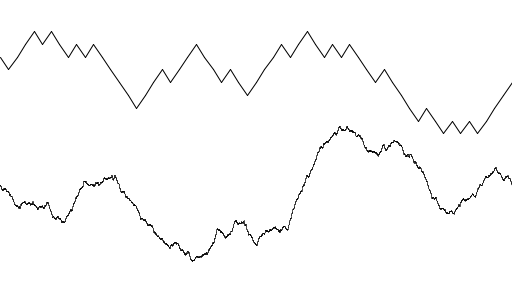
\includegraphics[height=0.25\textheight]{graphics/Gaussian.png}
\caption{An example of a random walk and a Brownian motion.}
\end{figure}

\end{frame}

\begin{frame}{Multiple random walks}
	
	\begin{itemize}
		
	\item If $S_{n+1} - S_n \in \{0, 1\}$, then $\{S_n\}_{n=1}^\infty$ is a \textcolor{red}{\textit{Bernoulli random walk}} 
	
	\item An \textcolor{red}{\textit{avoiding Bernoulli line ensemble}} $\mathfrak{L} = (L_1,\dots,L_k)$ consists of $k$ avoiding Bernoulli random walks on an interval $[T_0,T_1]$, such that $L_1(s) \geq L_2(s) \geq \cdots \geq L_k(s)$ for $s\in[T_0,T_1]$
	
	\end{itemize}
\[
	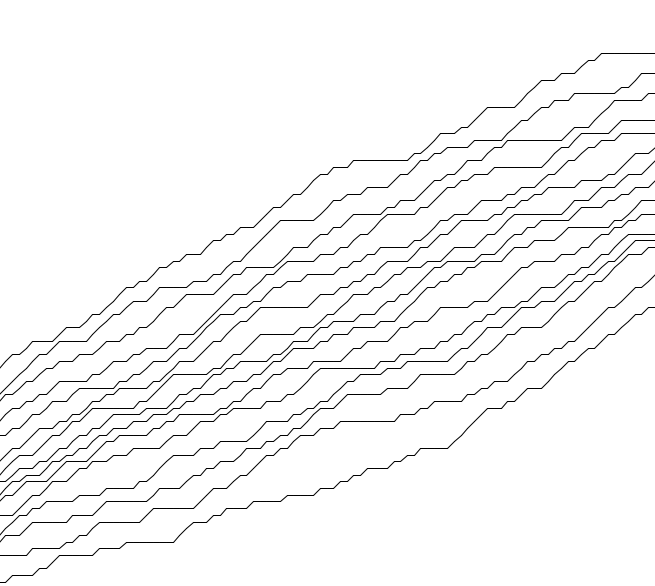
\includegraphics[height=0.5\textheight]{graphics/MultipleBernoulli.png}
\]
	\begin{itemize}
		\item Question: What does the limit look like as $k\to\infty$?
	\end{itemize}
\end{frame}

\begin{frame}{Airy Line Ensemble}
As $k \to \infty$, $k$ avoiding random walks are conjectured to converge to the \textit{\textcolor{red}{Airy line ensemble}} $\mathcal{A}$, and the top curve to the \textit{\textcolor{red}{Airy process}} $\mathcal{A}_1$
\begin{figure}
	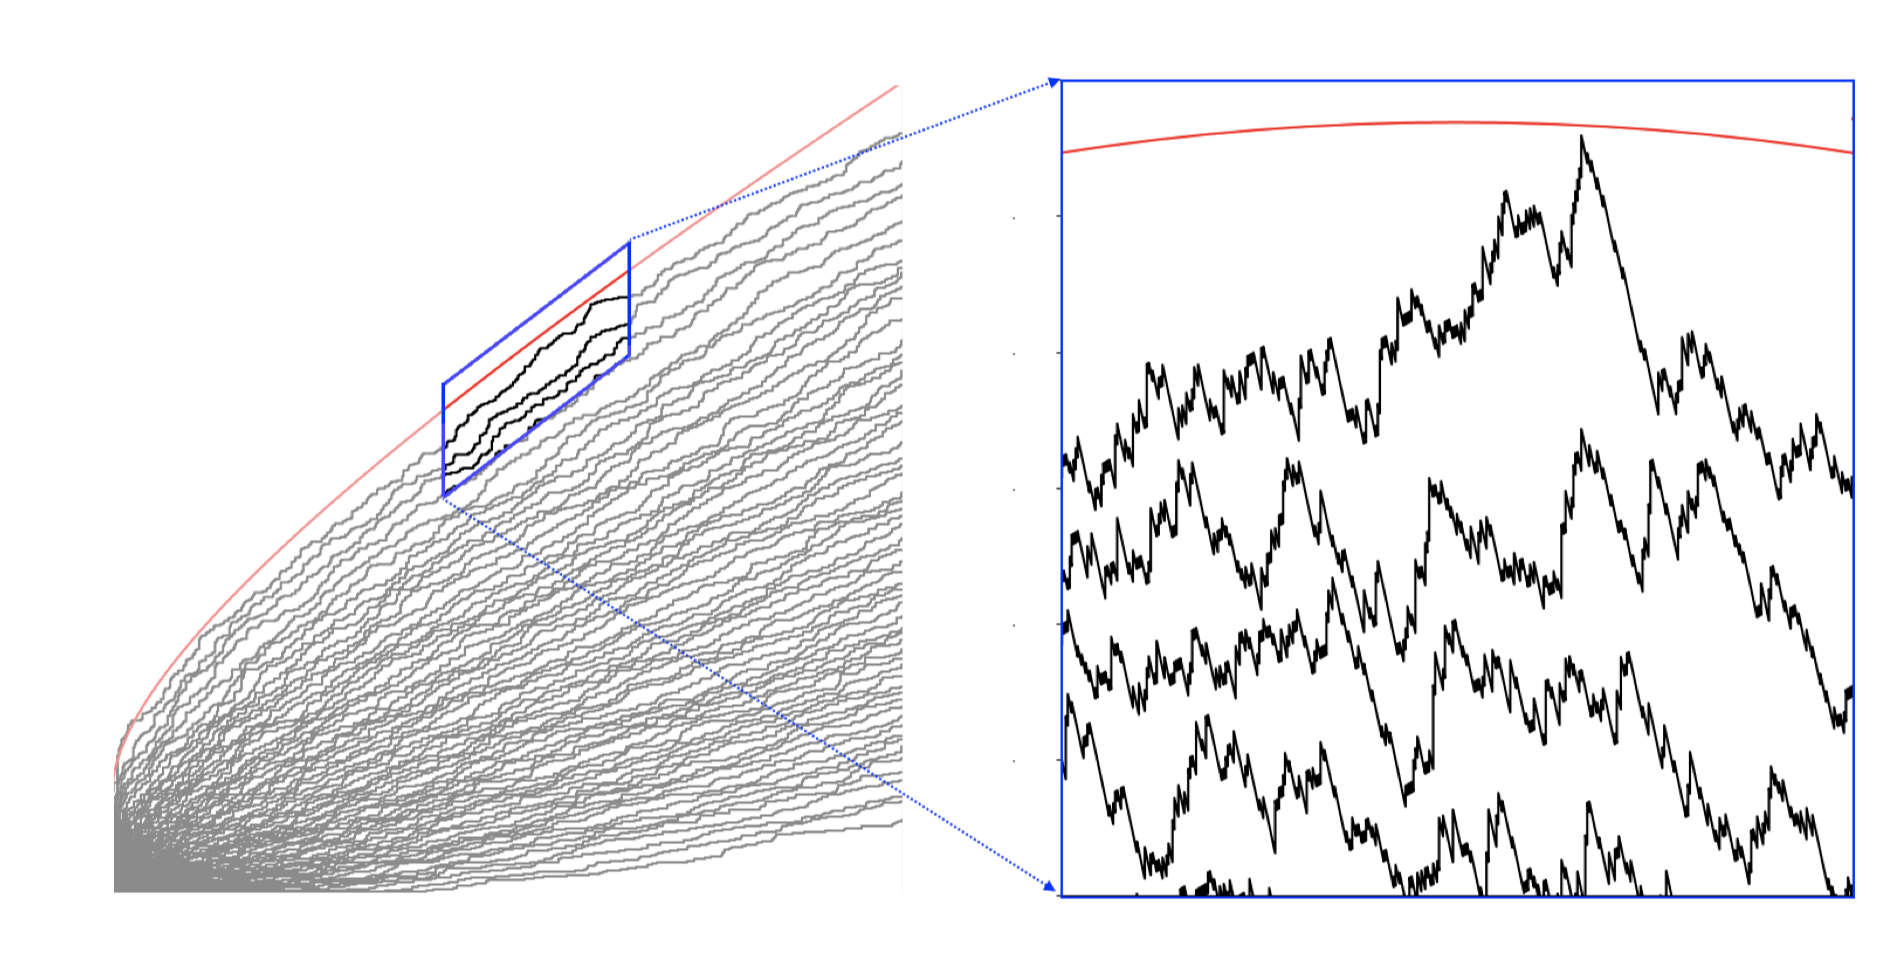
\includegraphics[height=0.45\textheight]{graphics/airy.png}
\end{figure}

\begin{itemize}
	
	\item Increasing the number of paths pushes us outside of the \textcolor{blue}{Gaussian universality class} and into the \textcolor{blue}{\textit{Kardar-Parisi-Zhang (KPZ) universality class}}
	
	\item Open problem: Show that ``generic" random walks with ``generic" initial conditions converge to the Airy line ensemble
	
	\item We consider this problem for Bernoulli random walks; the proof is only known if all walks start from 0
	
\end{itemize}
\end{frame}


\section{Convergence to Airy Line Ensemble (6-7 min)}

\begin{frame}{Convergence to the Airy Line Ensemble}
	
	Two sufficient conditions for convergence in distribution:
	\begin{itemize}
		
			\item \textcolor{red}{\textit{Finite dimensional}} convergence -- difficult, requires exact algebraic formulas
			
			\item \textcolor{blue}{\textit{Tightness}} (existence of weak subsequential limits) -- easier, more qualitative/analytic
	\end{itemize}

	We focused on \textcolor{blue}{tightness}, which we prove by controlling the maximum, the minimum, and the modulus of continuity
\begin{figure}
	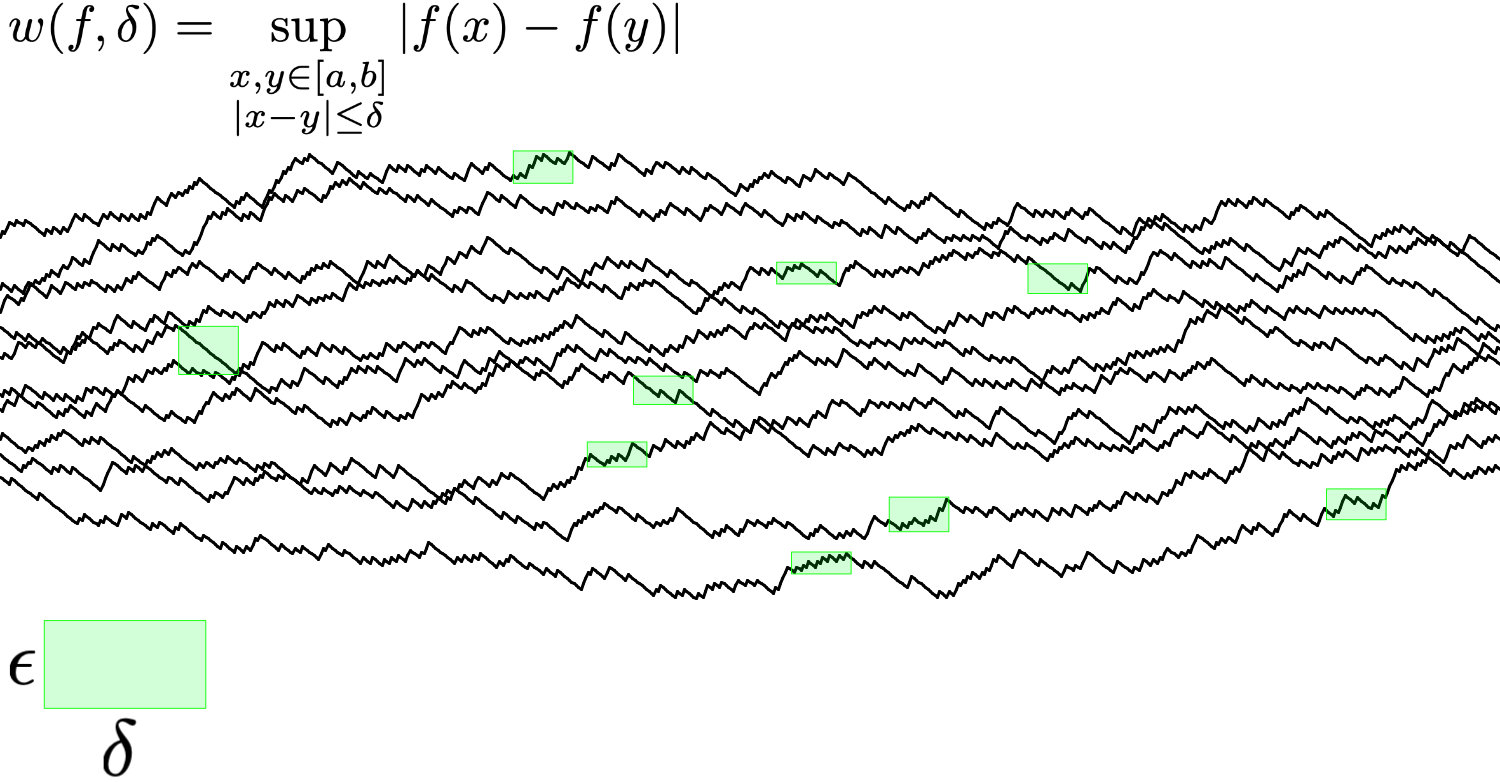
\includegraphics[height=0.55\textheight]{graphics/ModulusCont.jpg}
	\caption{The Modulus of Continuity}
\end{figure}

\end{frame}

\begin{frame}{Our Result}
\begin{theorem}[DFFSTWZ] Let $\{\mathfrak{L}^N = (L_1^N,\dots,L_k^N)\}_{N=1}^\infty$ be a sequence of $k$ avoiding Bernoulli random walks. Fix $p\in(0,1)$ and $\lambda > 0$, and suppose that for all $n\in\mathbb{Z}$ we have
\[
\lim_{N\to\infty} \mathbb{P}\big(L_1^{N}(nN^{2/3}) - pnN^{2/3} + \lambda n^2 N^{1/3} \leq N^{1/3} x \big) = F_{TW}(x).
\]
Then $\{\mathfrak{L}^N\}$ is a tight sequence.
\end{theorem}

\begin{itemize}
	\item $F_{TW}$ is the \textit{Tracy-Widom distribution} -- the one-point marginal for the Airy process
	
	\item {[Dauvergne-Nica-Vir\'{a}g '19]} showed that finite dimensional convergence of all curves implies tightness
	
	\item Our result shows that it suffices for the \textcolor{red}{top curve} to converge in the f.d. sense
\end{itemize}

\[
	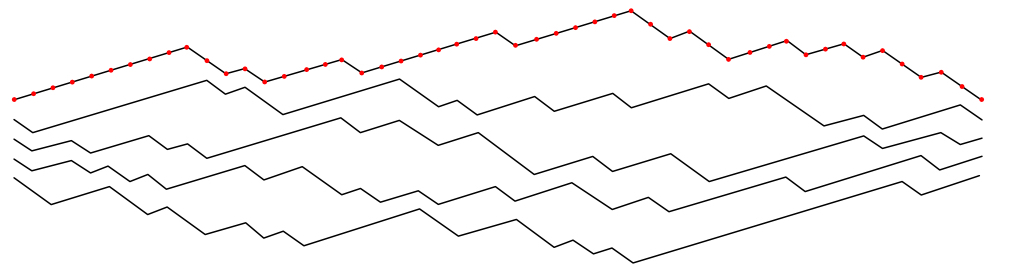
\includegraphics[scale=0.18]{graphics/ConvToTW.jpg}
\]
\end{frame}


\section{Section of Paper (7-9 min)}

\begin{frame} {History of the line ensembles}
	Arguments in this paper are inspired by 
	\begin{enumerate}
		\item \textit{Brownian Gibbs property for Airy line ensembles} [Corwin-Hammond '14] and \textit{KPZ line ensemble} [Corwin-Hammond '15], which address similar issues for {\color{red}continuous} line ensembles
		\item \textit{Transversal fluctuations of the ASEP, stochastic six vertex model, and Hall-Littlewood line ensembles} [Corwin-Dimitrov '17], which considers similar questions in a {\color{red}discrete} setting 
	\end{enumerate}
\end{frame}
\begin{frame}{Proving tightness}
	Recall that to show tightness, we want to control:
	\bigskip
	\begin{enumerate}
		\item \textbf{\textcolor{ForestGreen}{Minimum}} of bottom curve $\textcolor{ForestGreen}{L_k^N}$
		
		\bigskip
		
		\item \textbf{\textcolor{blue}{Maximum}} of top curve $\textcolor{blue}{L_1^N}$
		
		\bigskip
		
		\item \textbf{\textcolor{Fuchsia}{Modulus of continuity}} of each curve $\textcolor{Fuchsia}{L_i^N}$
		
		\bigskip
	\end{enumerate}
	We will focus on bounding the \textcolor{ForestGreen}{minimum}:
	
	\begin{lemma}[DFFSTWZ]
		Fix $r,\epsilon > 0$. Then there exist constants $M>0$ and $N_0\in\mathbb{N}$ such that for all $N\geq N_0$,
		\[
		\mathbb{P}\Big(\inf_{x\in[-r,r]} \big(L_k^N(xN^{2/3}) - pxN^{2/3}\big) < -MN^{1/3}\Big) < \epsilon.
		\]
	\end{lemma}
\end{frame}

\begin{frame}{Monotone coupling}
Lowering entry and exit data $\vec{x},\vec{y}$ for the curves $\implies$ curves shift down on whole interval [Corwin-Hammond '14]
\begin{center}
  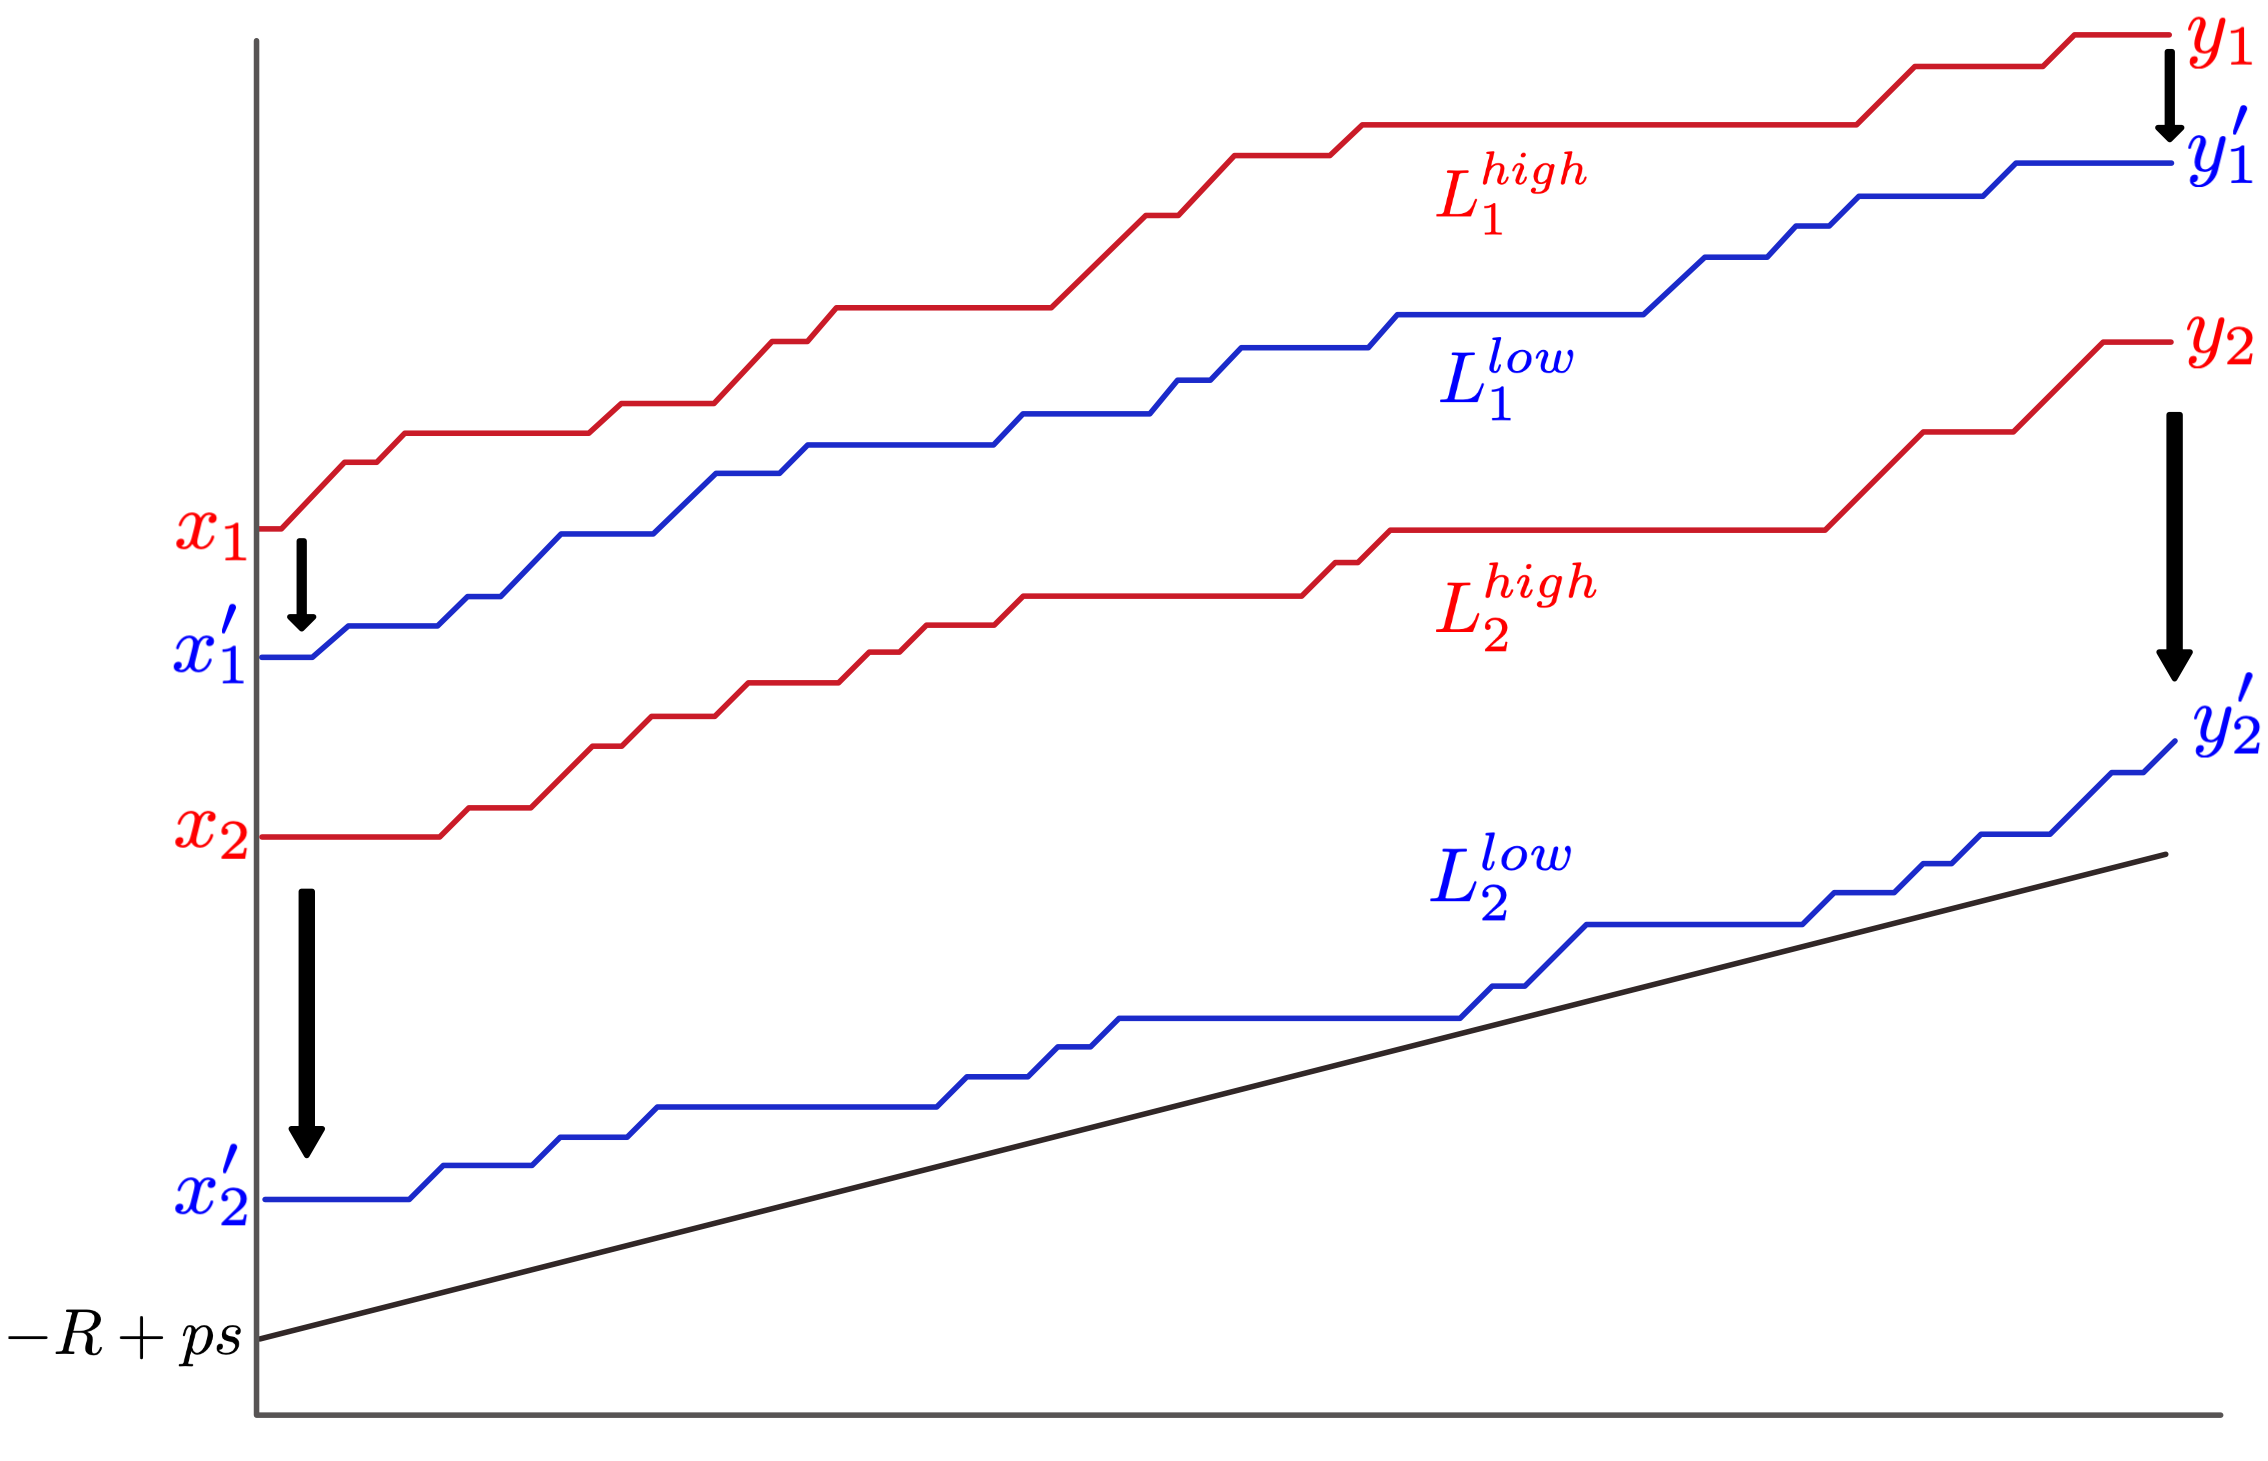
\includegraphics[scale=0.6]{graphics/monotonecoupling.png}{\kern 3em}
\end{center}
\begin{itemize}
	\item $\textcolor{red}{\mathfrak{L}^{high}}$ and $\textcolor{blue}{\mathfrak{L}^{low}}$ are ``coupled":
	\[
	\mathbb{P}(\textcolor{red}{L_k^{high}}(s) < -R) \leq \mathbb{P}(\textcolor{blue}{L_k^{low}}(s) < -R)
	\]
\end{itemize}
\end{frame}

\begin{frame}{Strong coupling}
	
A \textcolor{blue}{Bernoulli random walk} $\textcolor{blue}{\ell^{(N)}}$ on $[0,N]$ can be coupled with an ``exponentially close" \textcolor{red}{Brownian bridge} $\textcolor{red}{B^{(N)}}$ [Dimitrov-Wu '19] 
\[
  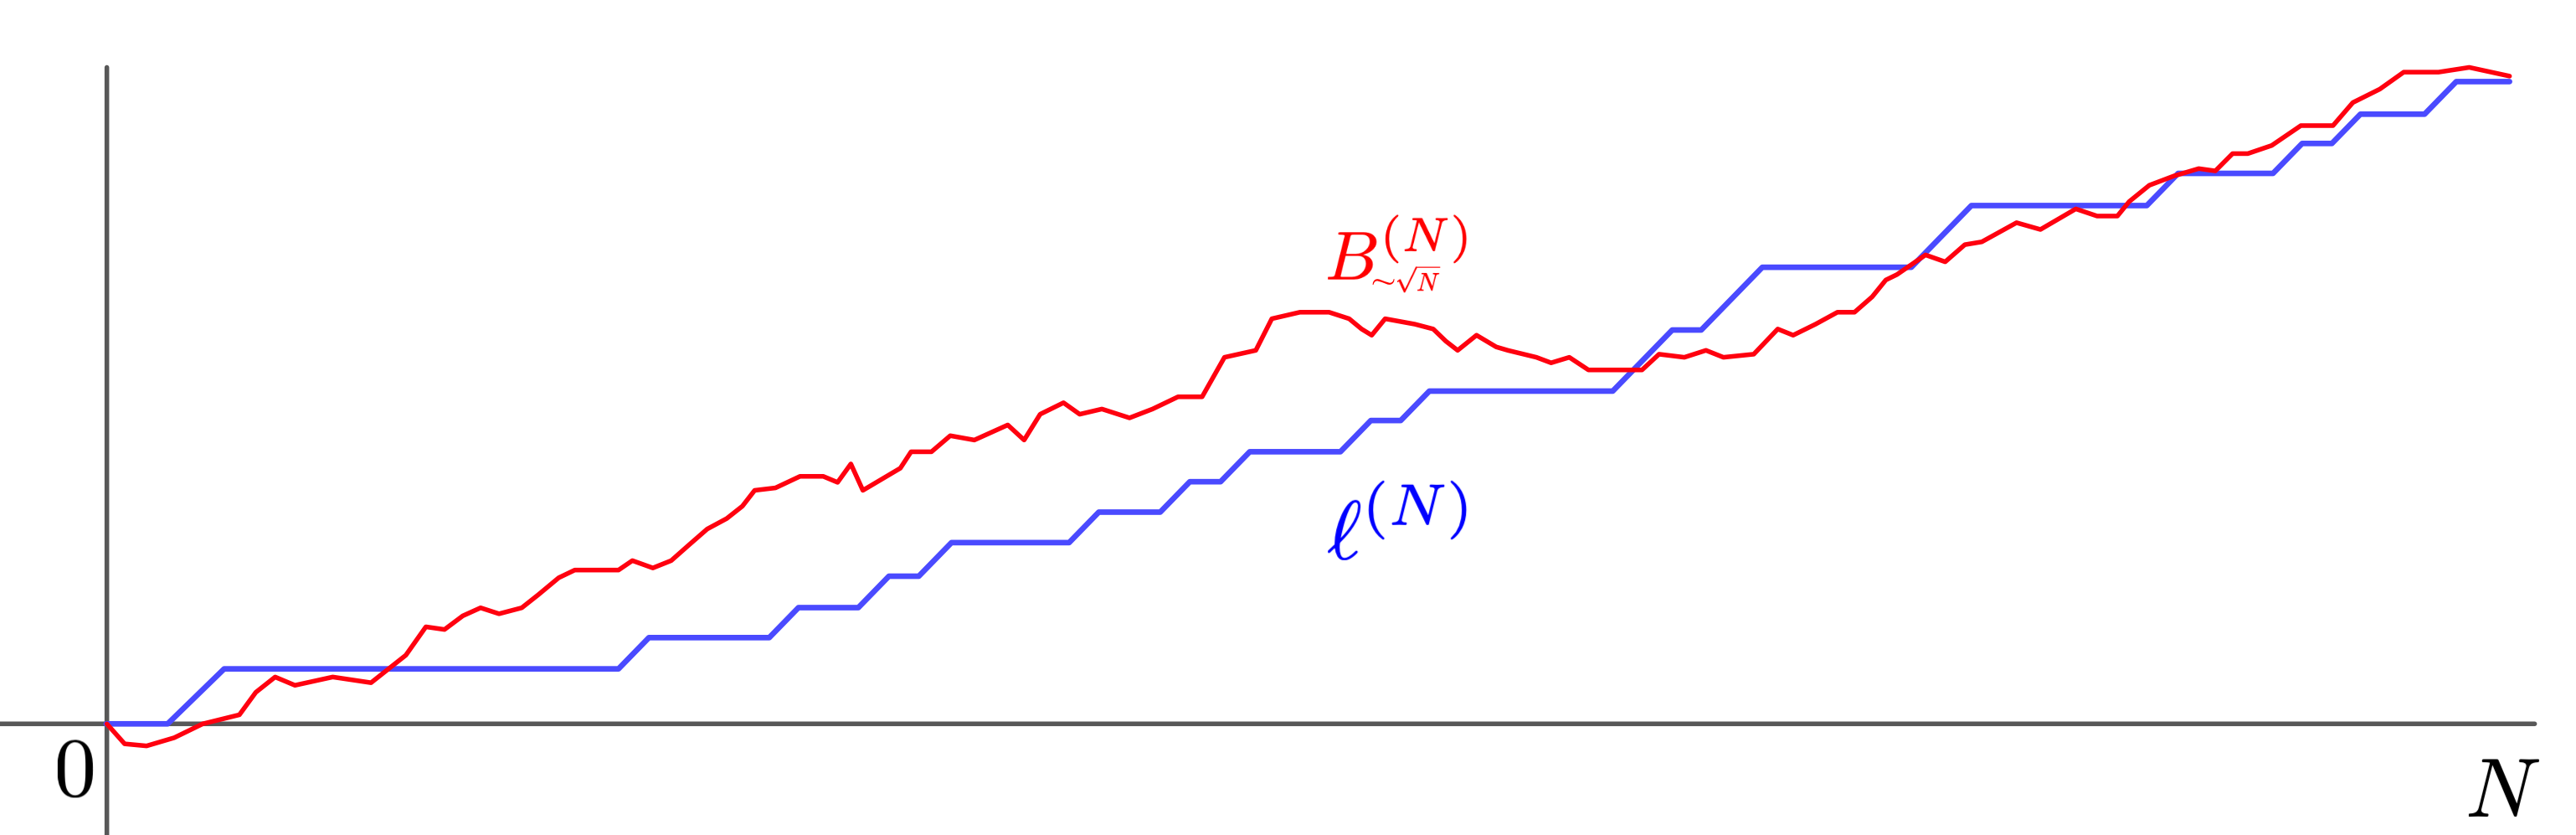
\includegraphics[width=\textwidth]{graphics/SCResult.png}
\]

\[
\mathbb{P}\Big( \sup_{s\in[0,N]} \abs*{\textcolor{blue}{\ell^{(N)}}(s) - \textcolor{red}{B^{(N)}}(s)} \geq M (\log N)^2 + x\Big) < Ke^{-Ax}
\]

\end{frame}


\begin{frame}{Controlling the minimum: pinning the bottom curve}
	
	\begin{lemma}[DFFSTWZ]
		For any $r,\epsilon > 0$, there exists $R>r$ and a constant $M>0$ so that for large $N$,
		\[
		\mathbb{P}\Big(\max_{x\in[r,R]} \big(L_k^N(xN^{2/3}) - \textcolor{red}{pxN^{2/3}}\big) < \textcolor{ForestGreen}{-MN^{1/3}}\Big) < \epsilon.
		\]
		The same is true of the maximum on $[-R,-r]$.
	\end{lemma}
	\[
	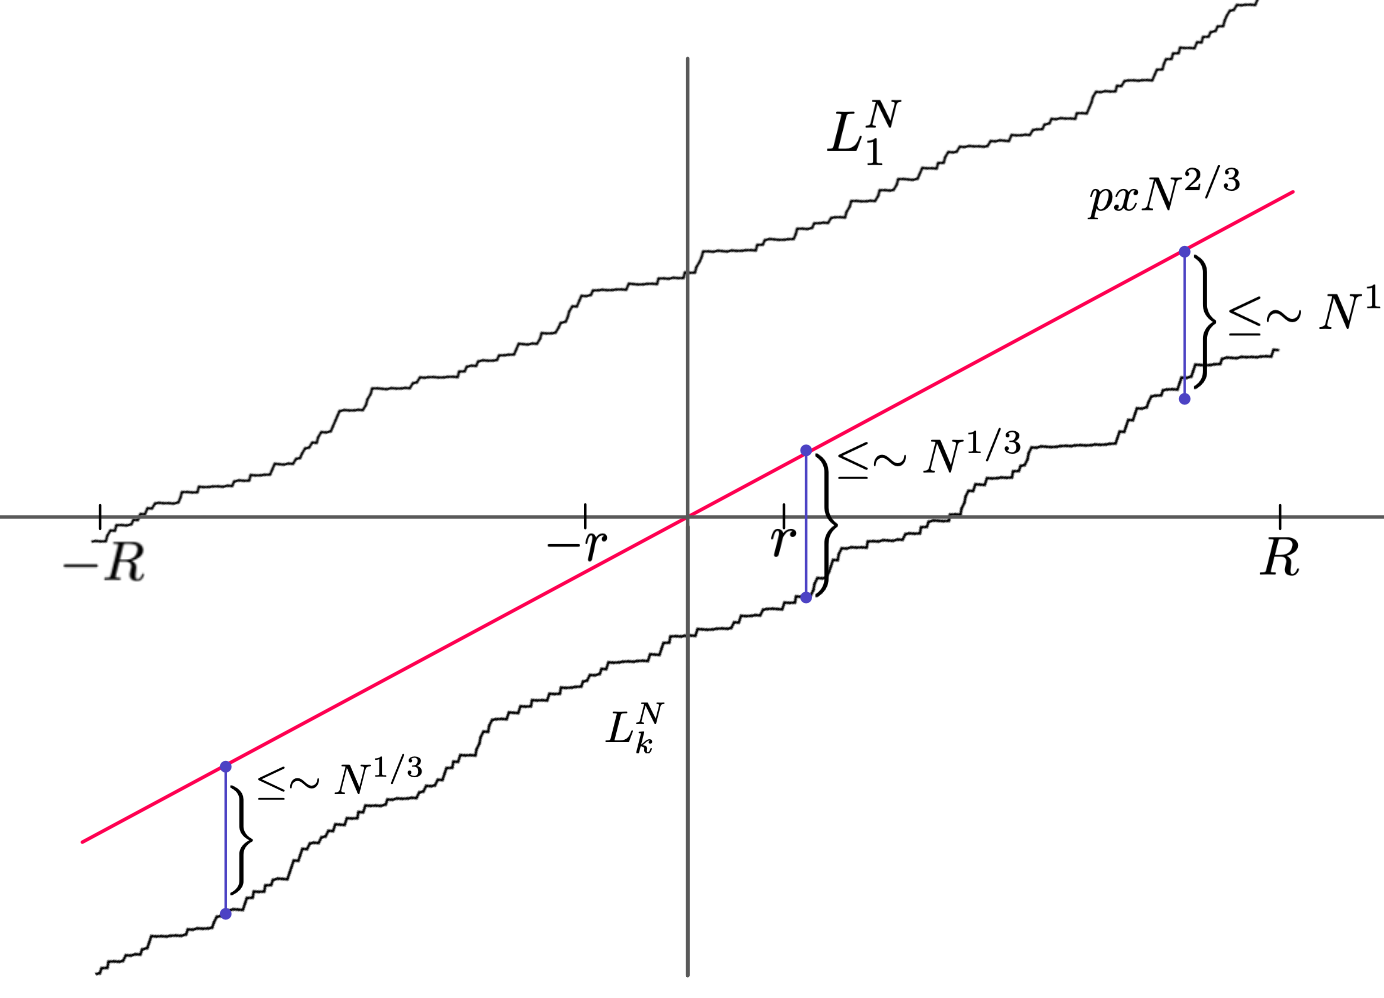
\includegraphics[scale=0.12]{graphics/min2.png}
	\]
	
	Couple $L_k^N$ with a Brownian bridge: if ``pinned" at two points in $[r,R]$ and $[-R,-r]$, it cannot be low on scale $N^{1/3}$ on $[-r,r]$
	
	
	
\end{frame}

\begin{frame}{Proving the pinning lemma}
	
	\begin{itemize}
		
		\item Recall our assumption:
		\[
		\mathbb{P}\Big(\textcolor{blue}{L_1^N}(nN^{2/3}) - pnN^{2/3} + \textcolor{blue}{\lambda n^2} N^{1/3} \leq xN^{1/3}\Big) \underset{N\to\infty}\longrightarrow F_{TW}(x)
		\]
		
		\item The top curve looks like a \textcolor{blue}{parabola} with an affine shift on large scales
		\begin{center}
		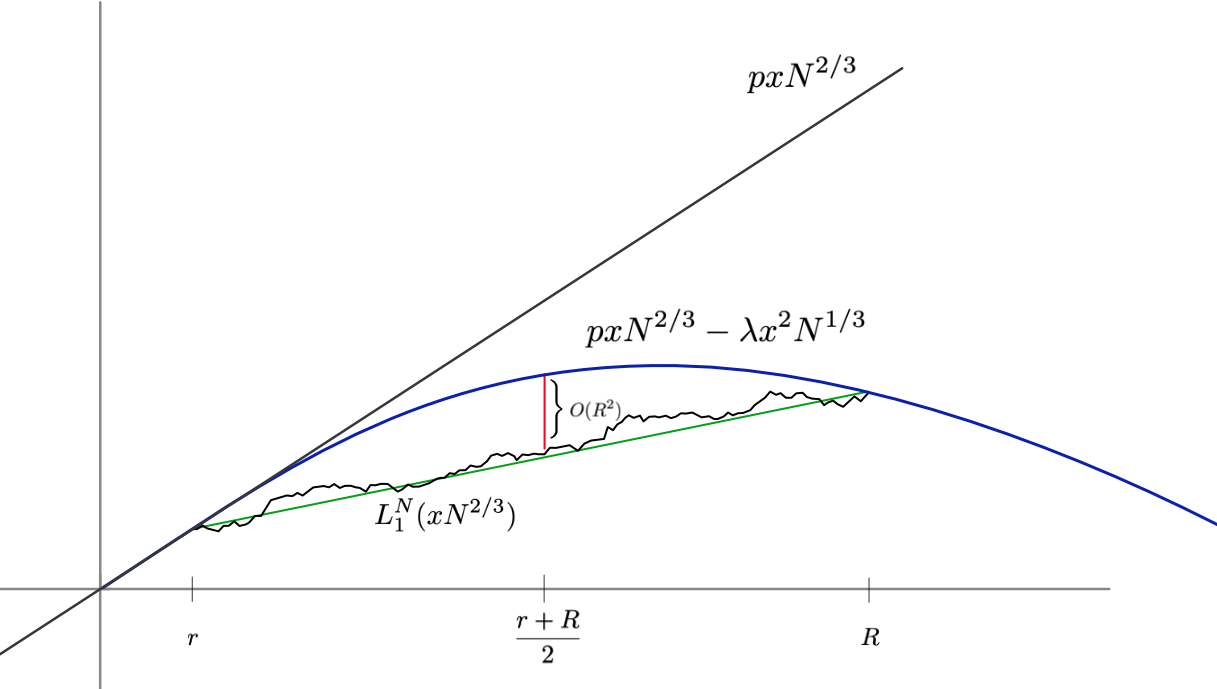
\includegraphics[scale=0.15]{graphics/parabola2.png}{\kern 4em}
		\end{center}
		
		\item Two curves: if $L_2^N$ is low on $[r,R]$, $L_1^N$ looks like a free Brownian bridge
		
		\[
		\textcolor{ForestGreen}{\lambda\Big(\frac{R^2+r^2}{2}\Big)} - \textcolor{blue}{\lambda\Big(\frac{R+r}{2}\Big)^2} = \lambda\,\frac{R^2+r^2-2rR}{4} = \textcolor{red}{O(R^2)}
		\]
		
		\item For large $R$, the top curve would be far from the parabola at the midpoint!
		
	\end{itemize}

\end{frame}


\end{document}
